%\title{LaTeX Portrait Poster Template}
%%%%%%%%%%%%%%%%%%%%%%%%%%%%%%%%%%%%%%%%%
% a0poster Portrait Poster
% LaTeX Template
% Version 1.0 (22/06/13)
%
% The a0poster class was created by:
% Gerlinde Kettl and Matthias Weiser (tex@kettl.de)
% 
% Adapter by Jens Buysse for Hogeschool Gent
% This template has been downloaded from:
% http://www.LaTeXTemplates.com
%
% License:
% CC BY-NC-SA 3.0 (http://creativecommons.org/licenses/by-nc-sa/3.0/)
%
%%%%%%%%%%%%%%%%%%%%%%%%%%%%%%%%%%%%%%%%%

%----------------------------------------------------------------------------------------
%	PACKAGES AND OTHER DOCUMENT CONFIGURATIONS
%----------------------------------------------------------------------------------------

\documentclass[a0,portrait]{a0poster}

\usepackage{multicol} % This is so we can have multiple columns of text side-by-side
\columnsep=100pt % This is the amount of white space between the columns in the poster
\columnseprule=3pt % This is the thickness of the black line between the columns in the poster

\usepackage[svgnames]{xcolor} % Specify colors by their 'svgnames', for a full list of all colors available see here: http://www.latextemplates.com/svgnames-colors

\usepackage{times} % Use the times font
%\usepackage{palatino} % Uncomment to use the Palatino font

\usepackage{graphicx} % Required for including images
\graphicspath{{figures/}} % Location of the graphics files
\usepackage{booktabs} % Top and bottom rules for table
\usepackage[font=small,labelfont=bf]{caption} % Required for specifying captions to tables and figures
\usepackage{amsfonts, amsmath, amsthm, amssymb} % For math fonts, symbols and environments
\usepackage{wrapfig} % Allows wrapping text around tables and figures
\usepackage[export]{adjustbox}

\usepackage{epigraph}

\begin{document}

%----------------------------------------------------------------------------------------
%	POSTER HEADER 
%----------------------------------------------------------------------------------------

% The header is divided into two boxes:
% The first is 75% wide and houses the title, subtitle, names, university/organization and contact information
% The second is 25% wide and houses a logo for your university/organization or a photo of you
% The widths of these boxes can be easily edited to accommodate your content as you see fit

\begin{minipage}[t]{0.75\linewidth}
\VeryHuge \color{HoGentAccent1} \textbf{Een gebruiker wegwijs maken doorheen een applicatie van aanzienlijke omvang} \color{Black}\\ % Title
\Huge\textit{Een studie met betrekking tot user experience, user interfaces en usability testing}\\[2.4cm] % Subtitle
\huge \textbf{Lierman Jakob, Maurau Bert, Samyn Karine}\\[0.5cm] % Author(s)
\huge Hogeschool Gent, Valentin Vaerwyckweg 1, 9000 Gent\\[0.4cm] % University/organization
\Large \texttt{jakob.lierman.y9252@student.hogent.be} \\
\end{minipage}
%
\begin{minipage}[t]{0.25\linewidth}

\includegraphics[width=13cm,right]{figures/HOGENT_Logo_Pos_rgb.png} 

\end{minipage}

\vspace{1cm} % A bit of extra whitespace between the header and poster content

%----------------------------------------------------------------------------------------

\begin{multicols}{2} % This is how many columns your poster will be broken into, a portrait poster is generally split into 2 columns

%----------------------------------------------------------------------------------------
%	ABSTRACT
%----------------------------------------------------------------------------------------

\color{HoGentAccent1} % Navy color for the abstract

\begin{abstract}
Elke gebruiker moet leren werken met de applicaties die hij of zij op zijn of haar toestel installeert. Men kan deze gebruiker helpen door middel van implementatie van learnability-elementen doorheen de software. De gebruiker kan op weg gezet worden door middel van een onboarding wanneer hij of zij de applicatie voor de eerste maal opent.

De grote meerderheid aan bedrijven en ontwikkelaars hebben echter de tijd of middelen niet om deze technieken zo geoptimaliseerd mogelijk uit te werken. Zo zijn deze vaak druk bezet met het halen van strakke deadlines om nieuwe functionaliteiten op punt te hebben dat de gebruikservaring vaak wat achterwege gelaten wordt.

Deze scriptie geeft duidelijkheid over de verschillende soorten onboarding en help-elementen en hoe deze best te gebruiken om een positief effect te hebben bij de eindgebruiker. Er wordt ook besproken hoe men best de implementatie van deze technieken test aan de hand van usability testing. Dit schrijven werd aangevuld met inzichten van ontwikkelaars.

Om het effect van learnability-elementen te meten werd er een usability test uitgevoerd met enkele participanten. Uit dit onderzoek resulteert dat het gebruik van deze elementen wel degelijk voordelig is, als en slechts als deze op de juiste manier verwerkt zijn doorheen de software. Elke software verschilt en voor elke software moet opnieuw bekeken worden waar men best hulp kan voorzien. Dit gaat vlot aan de hand van usability tests doorheen fases van de ontwikkeling.

De relatie tussen (het gebrek aan) in-app user training en de gebruiksduur en/of levensduur van de applicatie wordt aanbevolen als toekomstig onderzoek. Hierbij kan men deze proef als startpunt gebruiken met een gerichte applicatie en een steekproef waarbij elke participant interesse toont in de functionaliteiten van de applicatie.
\end{abstract}

\color{HoGentAccent1} 
\section*{Introductie}
\color{black}
\color{black}

\epigraph{If the user can't use it, it doesn't work.}{\textit{Susan Dray}}

In digitale tijden als deze is de vraag naar nieuwe software groot. Programmeurs en IT-bedrijven hebben hun handen vol. Zowat elke sector wil mee zijn met de digitale boot. Je komt hedendaags overal software tegen; de computer op het werk, de smartphone in je broekzak, het bedieningspaneel van een grote kraan, de kassa in de supermarkt, $\dots$ Je gebruikt hoogstwaarschijnlijk tal van software in het dagelijkse leven. Maar hoe leer je nu het best omgaan met deze computerprogramma's? Programma's bevatten vaak heel veel functies. Veel van deze functies blijven echter onbenut omdat de gebruiker niet voldoende begrijpt hoe deze functies in zijn werking treden. De programmeurs achter deze software hebben vaak hun handen al vol met het ineen knutselen van al deze functionaliteit waardoor zij zelf geen tijd hebben om te kijken hoe de eindgebruiker met deze functionaliteit omspringt.

\epigraph{How do I explain what I do at a party? The short version is that I say I humanize technology.}{\textit{Fred Beecher, Director of UX, The Nerdery}}

Hier komt de UX-designer aan bod. Een UX-designer zorgt er voor dat software bruikbaar is voor de eindgebruiker. Taken die zijn job omschrijven omvatten, maar zijn niet beperkt tot, het maken van prototypes, testen van (deel)producten bij gebruikers, observeren van gedrag van gebruikers op bepaalde functionaliteiten en stukken software, \textit{user flows} creëren en ook onderzoek doen naar de doelgebruiker. De UX-designer zal dus ook een flow creëren dat ervoor zorgt dat de gebruiker alle functionaliteit van de applicatie goed begrijpt en snel onder de knie heeft.

Eén van de bekendste implementaties hiervan is de ``onboarding''. Je komt vaak in contact met onboarding wanneer je de applicatie voor de eerste maal opstart. Zo'n onboarding kan zeer verschillend zijn van applicatie tot applicatie.
Er bestaan uiteraard meer manieren om de gebruiker de weg te wijzen doorheen software. Een simpele \textit{tooltip} of zelfs een help-pagina of leerplatform doet ook wonderen.

\subsection*{Probleemstelling}

Bij veel software-ontwikkelaars en -designers stelt de vraag zich frequent of een bepaalde implementatie van onboarding of in-app user training wel het gewenste effect bekomt. Er bestaan verscheidene manieren om dit in een applicatie te verwerken, om echter te weten of de ene manier een beter resultaat boekt dan de andere is een onderzoek nodig.

\color{Black} % DarkSlateGray color for the rest of the content
\color{HoGentAccent1} 
\section*{Experiment}
\color{black}

Om te bekijken of een implementatie van bepaalde learnability technieken invloed heeft op de eindgebruiker zullen er usability tests worden uitgevoerd bij testpersonen.

Bij dit experiment zal er vooral gefocust worden op laboratory testing. Dit wil zeggen dat de testpersoon de applicatie zal testen in het bijzijn van een moderator, maar niet strikt noodzakelijk in de omgeving waarin de applicatie in een reëel scenario gebruikt zou worden. De moderator noteert hierbij alle bevindingen van de testpersoon, alsook waar deze eventueel moeilijkheden ondervindt.

Het experiment zal uitgevoerd worden bij twee groepen. De ene groep krijgt een proof-of-concept applicatie waarin alle learnability technieken in verwerkt zijn. De controlegroep krijgt een applicatie zonder deze learnability elementen. Tijdens deze usability tests wordt van de testpersonen verwacht dat deze een reeks taken tot een goed einde proberen te brengen. Gedurende het experiment worden een aantal variabelen gemeten.

\color{HoGentAccent1} 
\section*{Proof-of-concept}
\color{black}

De proof-of-concept applicatie is een tool waarmee je je huidige spaardoelen kan bijhouden. Van zodra je de applicatie opent kan je een spaardoel toevoegen, je kan dit eventueel aanvullen met een bedrag dat je al gespaard hebt, een passende categorie en een deadline. Verder bestaat de applicatie uit drie onderdelen; je huidige spaardoelen, je voltooide spaardoelen en een handige calculator. Je huidige en voltooide spaardoelen worden weergegeven in een overzichtelijke lijst. Met de calculator kan je snel berekenen hoeveel je op dagelijkse basis moet sparen om een bepaalde deadline te halen of wanneer je je spaardoel zal behalen als je dagelijks een bepaald bedrag opzij legt.

\begin{center}\vspace{1cm}
	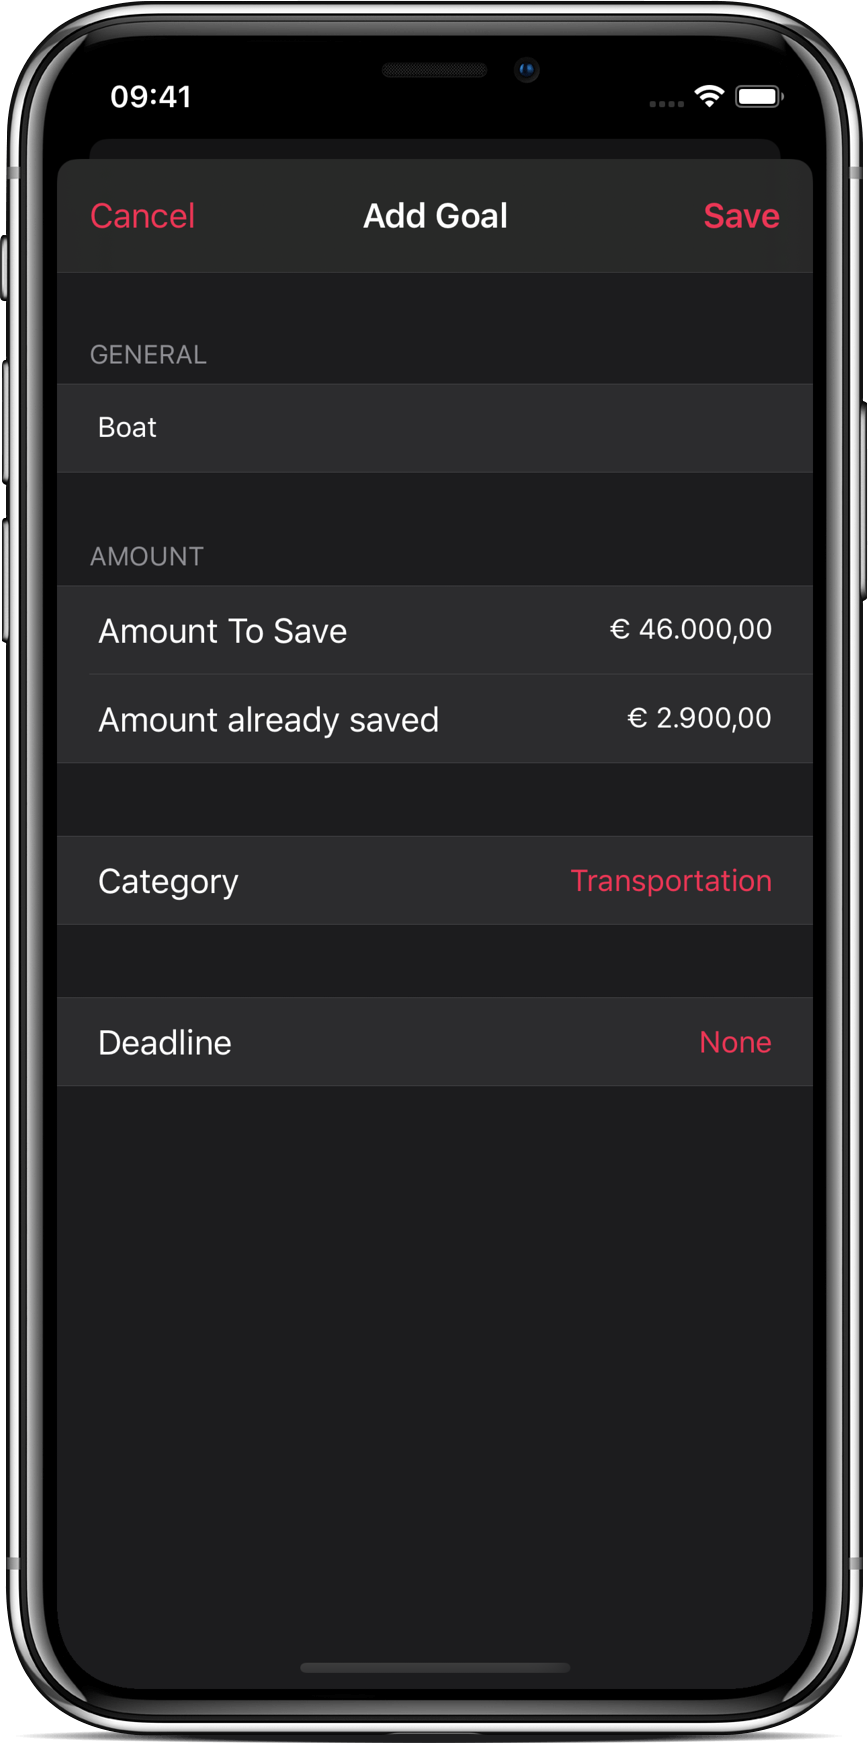
\includegraphics[width=.27\linewidth]{piggy-add-goal}
	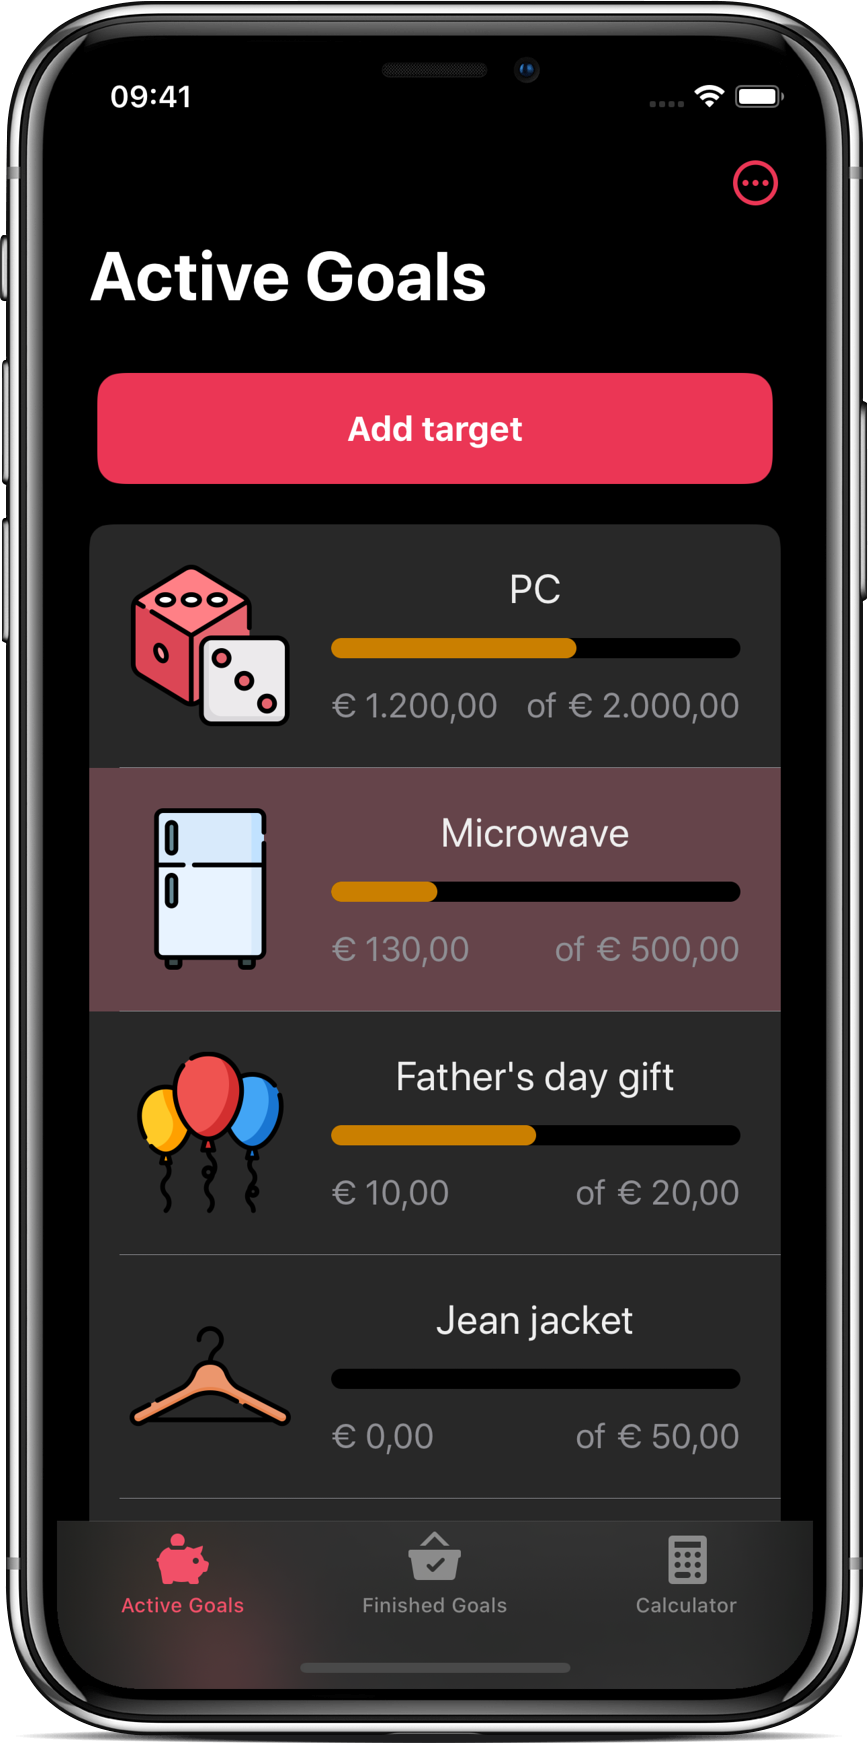
\includegraphics[width=.27\linewidth]{piggy-goals-list}
	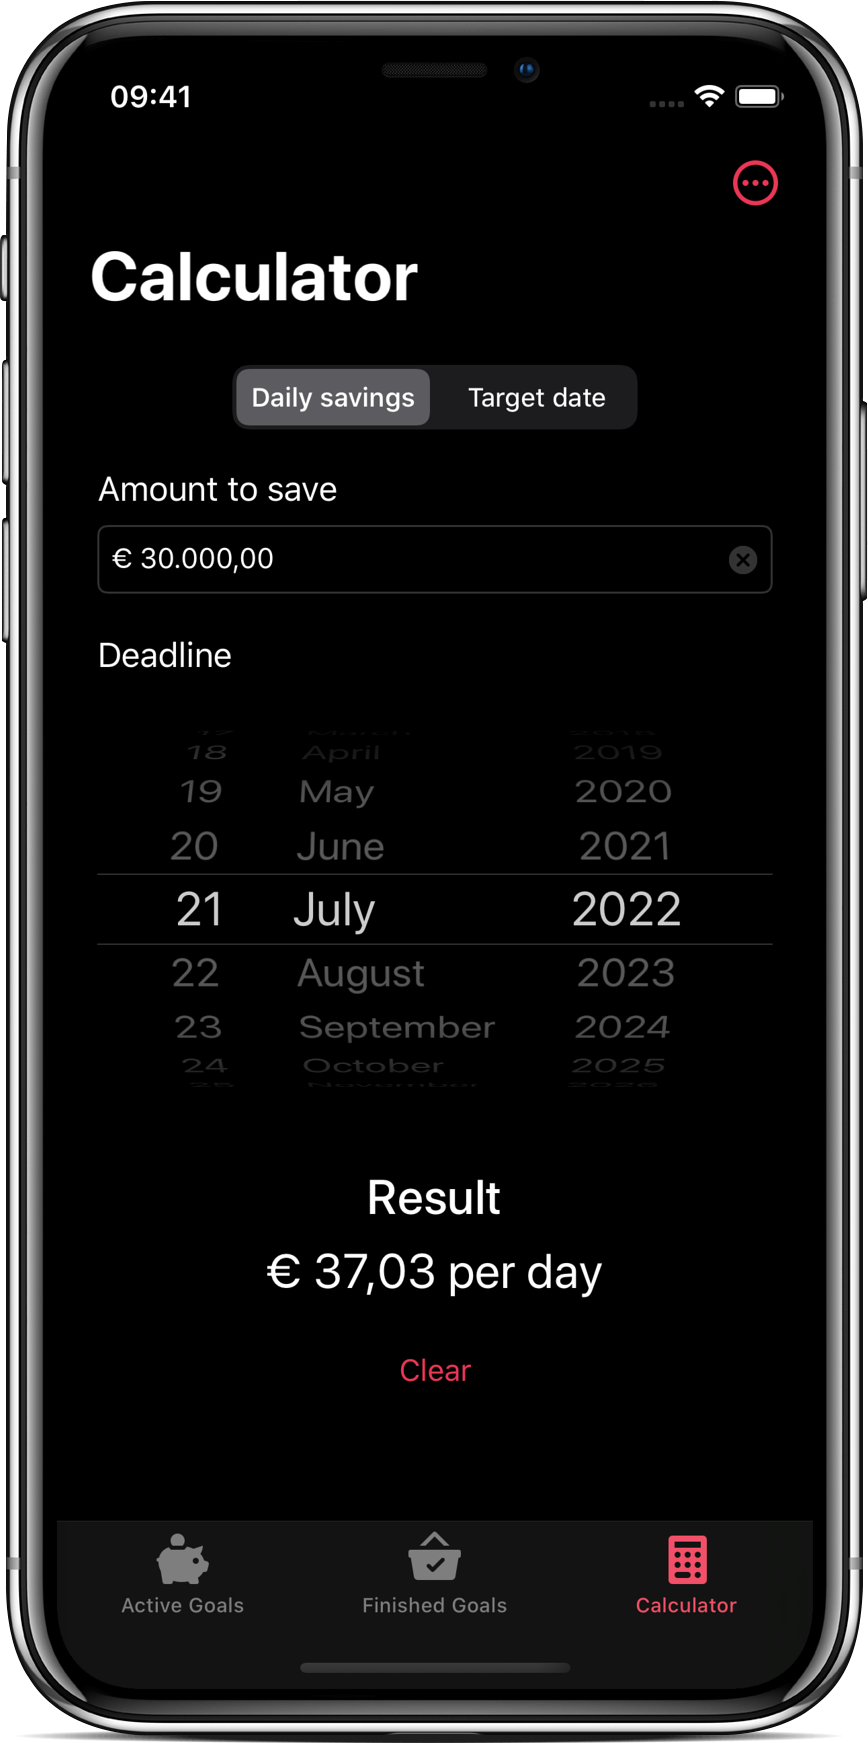
\includegraphics[width=.27\linewidth]{piggy-calculator}
	\captionof{figure}{\color{HoGentAccent5} Basisfunctionaliteiten van de proof-of-concept applicatie}
\end{center}\vspace{1cm}

Zoals vooraf aangehaald zullen er twee varianten van de proof-of-concept applicatie gemaakt worden. De ene variant bevat alle functionaliteiten maar hierbij is geen uitleg voorzien in de vorm van onboarding en/of in-app training.

\begin{center}\vspace{1cm}
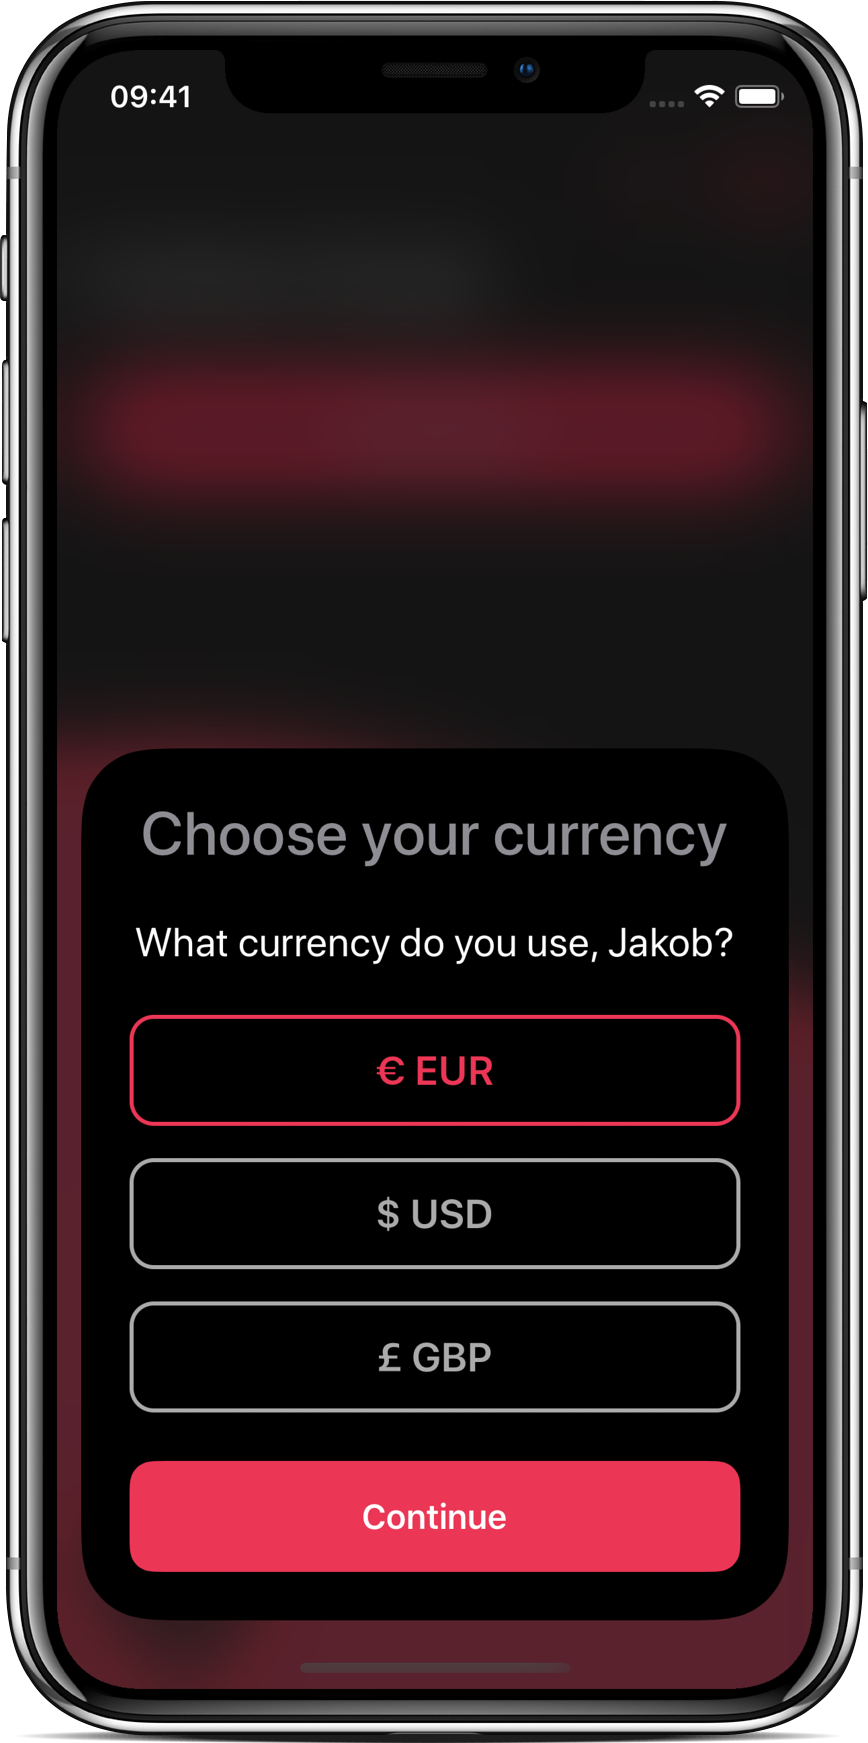
\includegraphics[width=.27\linewidth]{piggy-onboarding}
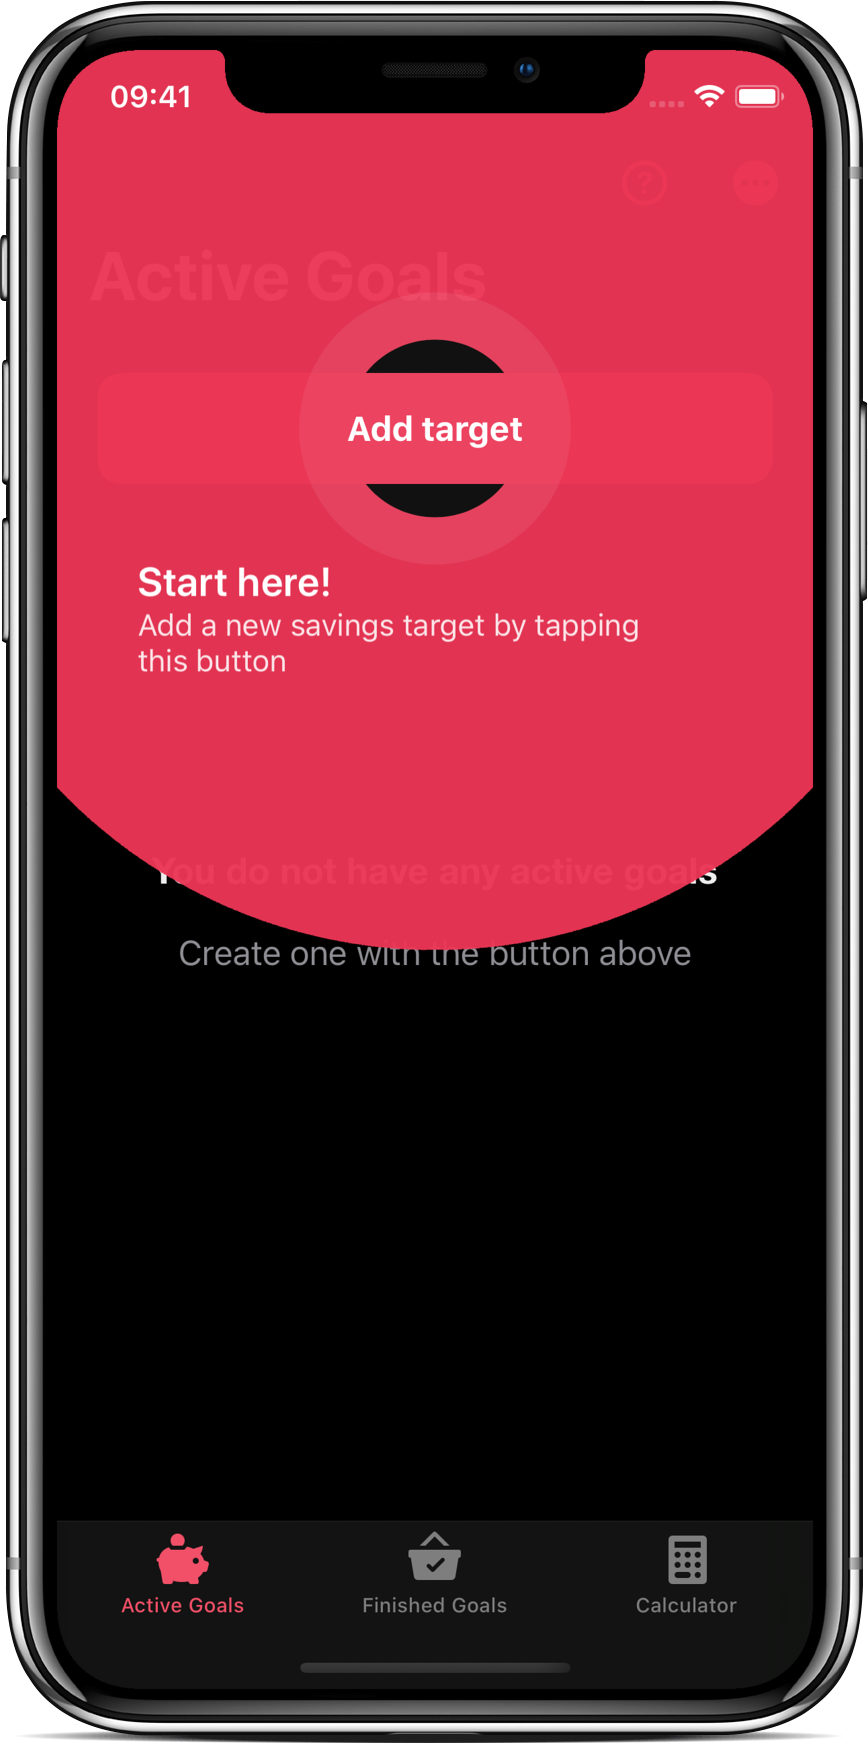
\includegraphics[width=.27\linewidth]{piggy-showcase}
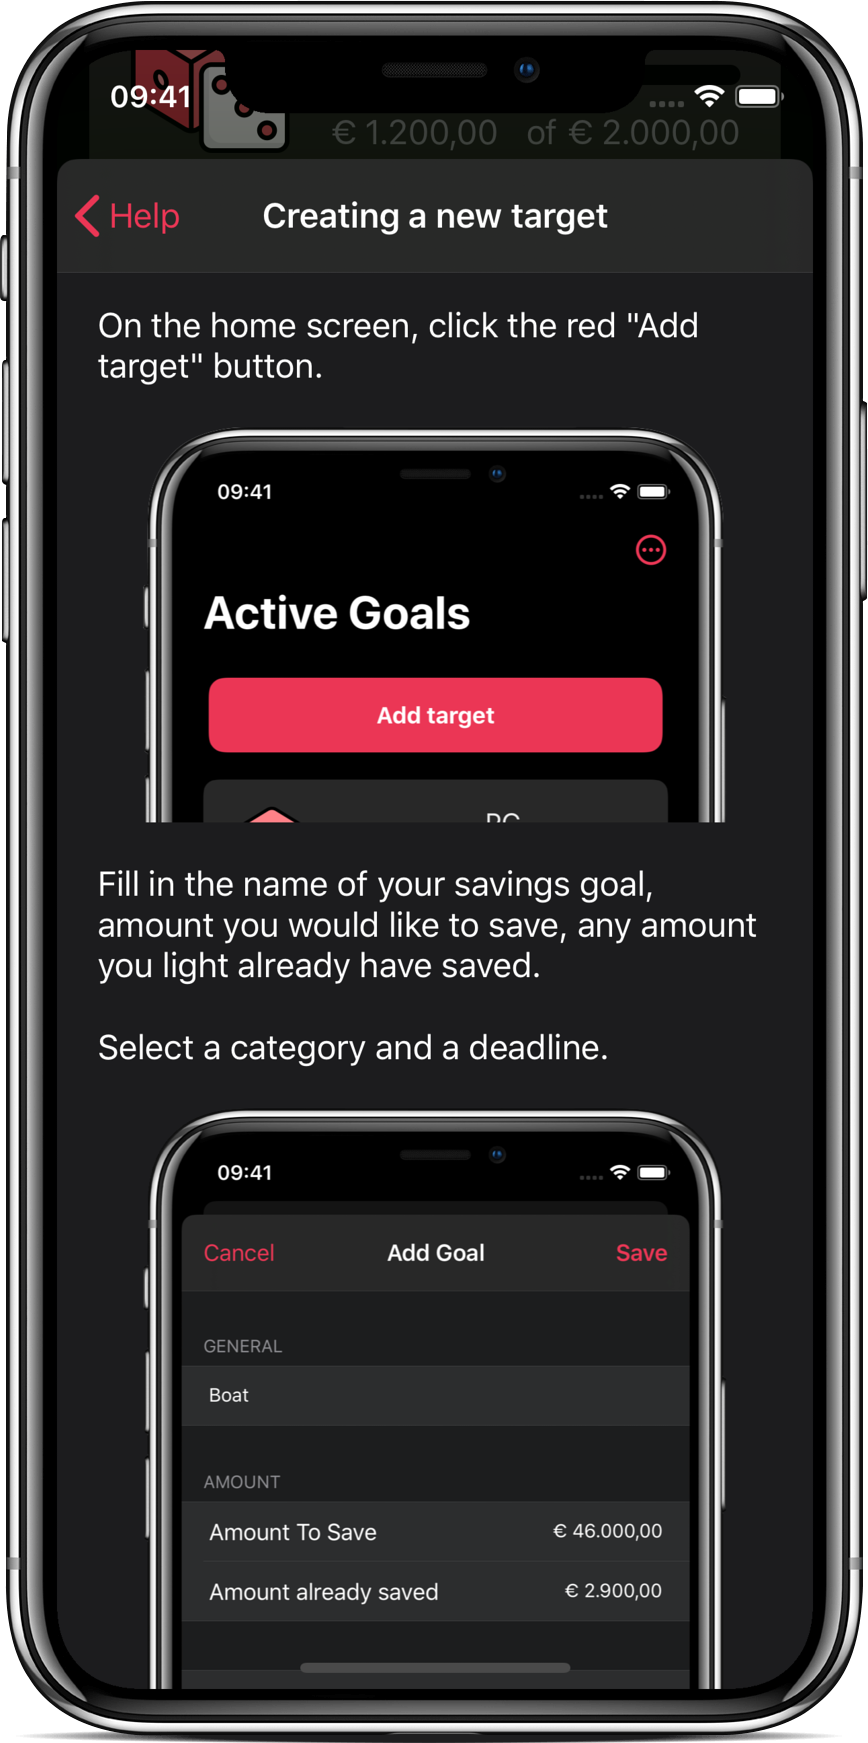
\includegraphics[width=.27\linewidth]{piggy-help-article}
\captionof{figure}{\color{HoGentAccent5} Een rondleiding doorheen de proof-of-concept applicatie}
\end{center}\vspace{1cm}

\color{HoGentAccent1} 
\section*{Conclusies}
\color{black}

De resultaten van deze proef gaven aan dat de learnability-elementen zeker hun nut hebben. Echter moet men zeer voorzichtig omspringen met waar en wanneer men deze plaatst. Zoals vooraf werd besproken is het belangrijk om zich te beperken tot de essentie, een gebruiker leert de details van de applicatie pas achteraf kennen. Zo wordt de gebruiker niet meteen overspoelt met informatie. Frequent de applicatie laten testen om zo te bekijken waar er hulp moet voorzien worden, is één van de belangrijkste stappen bij het implementeren van learnability in software.

\color{HoGentAccent1} 
\section*{Toekomstig onderzoek}
\color{black}

Er bestaan verschillende technieken om onboarding op een correcte manier te implementeren. Niet elke techniek kan voor elke applicatie of use case gebruikt worden. De ontwikkelaar van de software bekijkt best welke technieken geschikt zijn voor zijn of haar specifieke use case. Deze verschillen in UX voor verschillende applicaties kunnen eventueel onderzocht worden in een verder onderzoek.

Er werd voor deze applicatie geen significante relatie gevonden tussen (het gebrek aan) in-app user training en de gebruiksduur en/of levensduur van de applicatie. Wanneer een bedrijf hun software test bij gebruikers die ook effectief een meerwaarde hebben aan de functionaliteiten van deze software kan dit resultaat met hoogste waarschijnlijkheid variëren. Dit kan eventueel bewezen worden in een verder onderzoek.

\end{multicols}
\end{document}